%%%%%%   TIPO DE DOCUMEN%TO: Reporte   %%%%%%
\documentclass[letterpaper,11pt]{report}
%%%%%%%%%%%%%%%%%%%%%%%%%%%%%%%%%%%%%%%%%%%%

%%%%%%%   PAQUETES   %%%%%%%
\usepackage[spanish]{babel}
\usepackage{graphicx}
\usepackage[utf8]{inputenc}
%%%%%%%%%%%%%%%%%%%%%%%%%%%%

%%%%%%%%%%%%%%%%%%%%%%%%%%%%%%%%%%%%%%%%
%%%%%%%   INICIO DEL DOCUMENTO   %%%%%%%
%%%%%%%%%%%%%%%%%%%%%%%%%%%%%%%%%%%%%%%%
\begin{document}

    %%%%%%% Renombrar en espaNol %%%%%%
    \renewcommand{\tablename}{Tabla} %Escribe Tabla en lugar de Cuadro
    \renewcommand{\listtablename}{\'Indice de tablas} %Escribe Indeice de tablas en lugar de Indice de cuadros

    %%%%%%%   PORTADA   y RESUMEN   %%%%%%% Este es el contenido agregado de la secci\'on 2.

    %%%%%%%%%%%%%%%%%%%%%%%%%%%%%
%%%%%      PORTADA      %%%%%
%%%%%%%%%%%%%%%%%%%%%%%%%%%%%

\begin{titlepage}

    \centering %Todo centrado

    %%%%  LOGO DE LA ESCUELA   %%%%
    
\includegraphics[scale=0.17]{imagenes/escom-ipn} %Imagen para portada
    %%%%  NOMBRE DE LA ESCUELA   %%%%
    \LARGE{\\ Instituto Polit\'ecnico Nacional}
    \LARGE{\\ Escuela Superior de C\'omputo}
    
    \vspace{1cm} %Espacio vertical

    %%%%  TITULO Y NÚMERO DE TRABAJO   %%%%
    \LARGE \textbf{Augmented Reality Furniture (ARF)}
    \LARGE {\\ TT2018-A002}

    \vspace{1cm} %Espacio vertical

    \LARGE \textit{Que para cumplir con la opción de titulación curricular en la carrera de:}
    \LARGE \textbf{\\ Ingeniería en Sistemas Computacionales}

    \vspace{1cm} %Espacio vertical

    %%%%   ALUMNOS   %%%%
   \textit{Presentan}\\
    Cabello Acosta Gerardo Aramis\\
    Carrillo Mendoza Martín Alejandro \\
    Del Pilar Morales Saúl

    \vspace{1cm} %Espacio vertical

    %%%%   Directores   %%%%
   \textit{Directores}\\
    M. en C. Vélez Saldaña Ulises. \bigskip  \\
    M. en C. José David Ortega Pacheco. \bigskip  
\end{titlepage} %incluye el archivo portada.tex
    %%%%%%%%%%%%%%%%%%%%%%%
%%%%    RESUMEN    %%%%
%%%%%%%%%%%%%%%%%%%%%%%

\begin{abstract}

  Aquí va el resumen general del documento de trabajo terminal.

\end{abstract}
 %Incluir resumen del documento (resumen.tex)

    %%%%%%%   INCLUIR ENCABEZADOS EN INDICES Y CAPITULOS   %%%%%%%
    \pagestyle{headings}

    %%%%%%%   NUMERACION EN CONTENIDO E INDICE DE TABLAS Y FIGURAS   %%%%%%%
    \pagenumbering{roman} %NUmeros romanos
    %\setcounter{page}{1} %Comienza en I por default, aquI se puedo modificar

    %%%%%%   INCLUIR CONTENIDO, INDICE DE FIGURAS E INDICE DE TABLAS   %%%%%%
    \tableofcontents
    \listoffigures
    \listoftables

    %%%%%%%   NUMERACION EN CAPITULOS   %%%%%%%
    \clearpage %Para iniciar con los arAbigos
    \pagenumbering{arabic} %Numeros arabigos
    %\setcounter{page}{1} %Comienza en 1 por default, aquI se puede modificar

    %%%%%%%   INCLUYE CAPITULOS Y SECCIONES   %%%%%%%
    \chapter{Introducci\'on}

En éste capítulo se define el contexto del trabajo terminal, el problema que vamos a abordar y por qué lo vamos a resolver, cuáles son nuestros objetivos y cómo vamos a lograr solucionar el problema planteado. También está descrito el trabajo previo (estado del arte) el cual aborda la problemática que escogimos
	   \section{Contexto de trabajo}

Actualmente vivimos en un entorno dominado por la tecnología; día a día se desarrollan nuevas herramientas con el fin de ayudar al ser humano a realizar tareas de una forma más fácil y eficiente, como los HMD (Head-mounted Display)\cite{B15}.


Por otro lado también nos encontramos en una época donde el diseño es un área de gran importancia en cualquier sector del mercado, por ejemplo, un buen diseño web en un sitio es fundamental lograr que un producto se logre vender o difundir, un buen diseño gráfico en campañas de marketing asegura más clientes; de igual forma nos encontramos con el diseño de interiores. Para esta última área se suelen contratar diseñadores de interiores profesionales para lograr que los espacios interiores de un inmueble consigan tal armonía que mejoren la calidad de vida de quienes lo habitan y además generen un impacto en las personas que usan éstas habitaciones.\par
El diseño de interiores profesional no sigue un proceso estandarizado, sin embargo a nivel general podemos ubicar las siguientes etapas:

\begin{itemize}
	\item El cliente acude con un diseñador de interiores profesional, quien acude al domicilio para conocer las condiciones del inmueble y conocer las necesidades y presupuesto del cliente.
	\item Conociendo estos dos puntos el diseñador hace un análisis de viabilidad que se compone de un análisis presupuestal y la definición del alcance del diseño.
	\item El diseñador le muestra esta información al cliente para que la apruebe, en caso de no ser así, el proyecto es considerado como no viable.
	\item De ser viable el diseñador de interiores genera un calendario previo de actividades donde programa el cumplimiento de los requerimientos del cliente en determinadas fechas.
	\item Si el cliente aprueba la propuesta de calendario, el diseñador se dispone a realizar el \textbf{proceso de propuesta de diseño de interiores} con el objetivo de mostrarle al cliente el resultado final previo de la obra antes de que sea realizada, esta propuesta puede mostrarse de varias formas como fotografías con fotomontajes, una explicación verbal con fotografías de apoyo (de muebles o habitaciones ya decoradas) o un modelado tridimensional del resultado de la obra; se suele usar un modelado tridimensional pues es lo más cercano a la realidad que se le puede mostrar al cliente. Si el cliente no aprueba la propuesta de calendario, se debe volver a realizar el análisis de viabilidad para ajustarse a las necesidades y presupuesto del cliente.
	\item El diseñador le muestra la propuesta de diseño al cliente y si esta es aceptada, se inicia el desarrollo de la obra con base en las fechas establecidas.
	\item Finalmente el diseñador entrega la obra al cliente y termina el proceso de diseño de interiores.
\end{itemize}

El proceso completo anteriormente descrito se puede observar en la figura 1.1 a través de un diagrama de proceso de negocio, en las figuras 1.2 y 1.3 se muestra el diagrama segmentado para una mejor lectura del mismo, y en la figura 1.4 puede observar el \textbf{proceso de propuesta de diseño de interiores}.\par
Teniendo a la mano una gran diversidad de herramientas tecnológicas, podemos usar estos elementos para lograr que el diseño de interiores sea más sencillo y rápido, tanto para un diseñador de interiores que vaya a realizar una obra para algún cliente, como para alguien que desee diseñar o rediseñar su propio inmueble.
\newpage

\begin{figure}[!htbp]
	\centering
	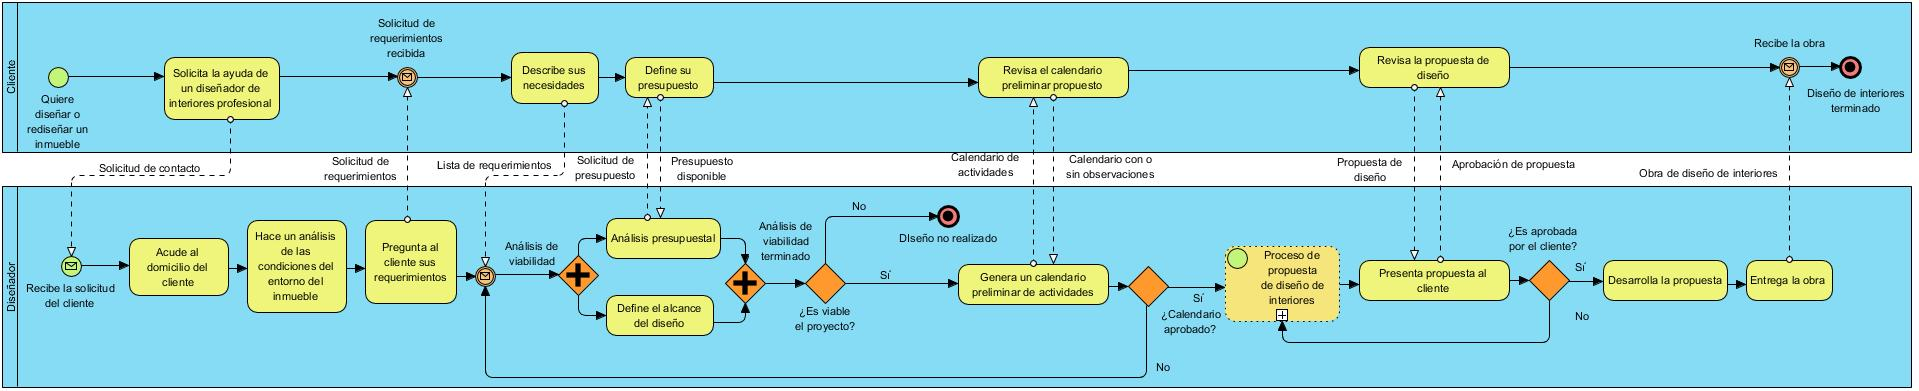
\includegraphics[width=20cm,angle=270,origin=c]{imagenes/marcoteorico/bpmn/proceso_full.jpg}
	\caption{Modelo del proceso de diseño de interiores (Completo).}
	\label{fig:bpmn_antes}
\end{figure}
\newpage

\begin{figure}[!htbp]
	\centering
	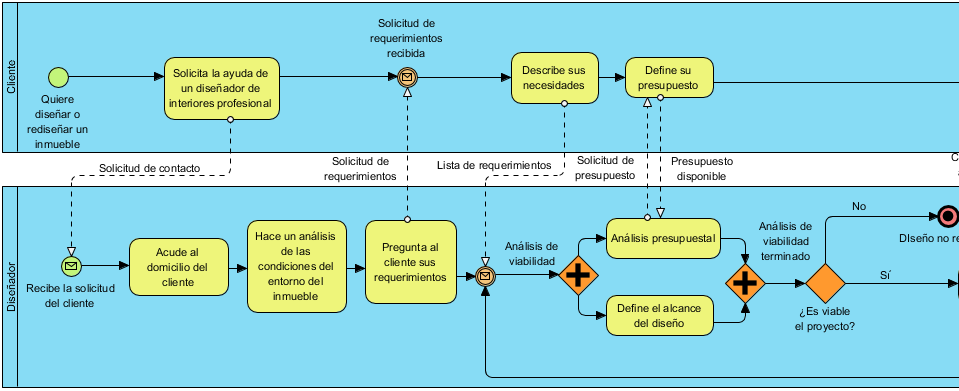
\includegraphics[width=19cm,angle=270,origin=c]{imagenes/marcoteorico/bpmn/proceso_01_01_left.png}
	\caption{Modelo del proceso de diseño de interiores (Segmento I).}
	\label{fig:bpmn_antes}
\end{figure}
\newpage

\begin{figure}[!htbp]
	\centering
	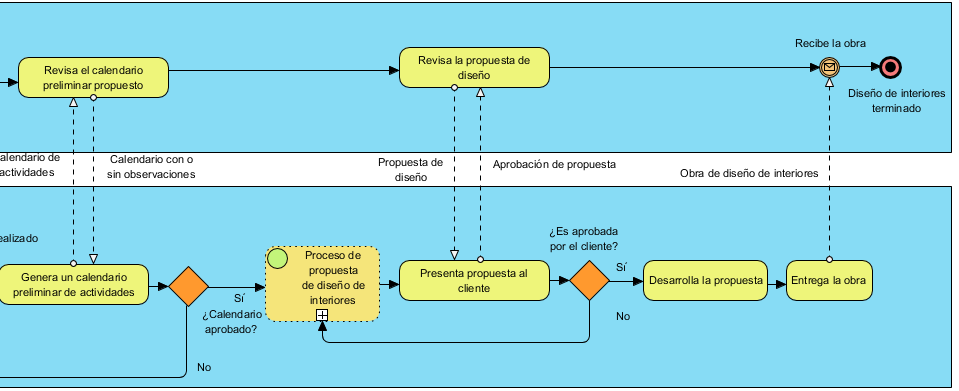
\includegraphics[width=19cm,angle=270,origin=c]{imagenes/marcoteorico/bpmn/proceso_02_01_left.png}
	\caption{Modelo del proceso de diseño de interiores (Segmento II).}
	\label{fig:bpmn_antes}
\end{figure}
\newpage

\begin{figure}[!htbp]
	\centering
	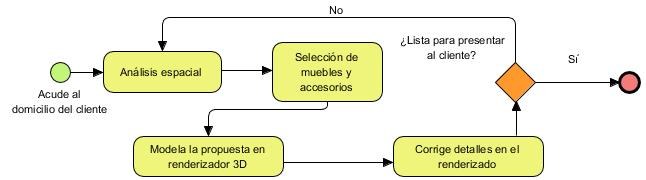
\includegraphics[width=16cm]{imagenes/marcoteorico/bpmn/subproceso.jpg}
	\caption{Subproceso de propuesta de diseño de interiores.}
	\label{fig:subproceso}
\end{figure}
\newpage
	   \section{Problemática}
El diseño de interiores para las personas en general, es un proceso complejo, tardado y tedioso, debido a la implicación del tratamiento superficial y el manejo del volúmen espacial, lo cual puede provocar pérdidas económicas y de tiempo por parte del cliente que compra un mueble y/o por parte de la tienda si se efectúa un proceso de devolución de producto dañando el prestigio de la tienda o sucursal asociada a la venta de estos muebles u objetos.

   
	   \section{Trabajo previo}
Las aplicaciones y proyectos que abordan el problema anteriormente descrito son:

\begin{enumerate}
	\item Canvas (iOS).
	\item Amazon App.
	\item Fingo.
	\item Ikea Place.
	\item TT 2012-B043. Realidad aumentada aplicada a la decoración de interiores.
\end{enumerate}

De forma colectiva, en tales aplicaciones pudimos notar las siguientes características:

\begin{enumerate}
	\item La cámara puede escanear una habitación para conocer los planos donde puede posicionar muebles.
	\item El usuario puede exportar el escaneo tridimensional de una habitación para usarlo en AutoCAD.
	\item Mediante realidad aumentada el usuario puede posicionar un objeto a donde enfoque la cámara del celular.
	\item Existe una posición relativa de los objetos, es decir, si el celular se mueve el objeto permanece en la misma posición.
	\item Se requiere un hardware especial además del dispositivo móvil.
\end{enumerate}

Cabe destacar que Fingo y el TT 2012-B043 utilizan marcadores físicos, colocados en el suelo, sobre los cuales se superponen los objetos tridimensionales, lo cual limita su uso, dado que son dependientes de un elemento externo.\par
Por otro lado, encontramos características que consideramos importantes para resolver el problema planteado, pero ninguna de las aplicaciones anteriores las posee, como son:


\begin{enumerate}
	%\item No están enfocadas a e-Commerce
	\item No existe un gran repertorio de submodelos de objetos
	\item No poseen valores agregados en los objetos en general, por ejemplo, que se muestre el costo de un producto.
	\item No muestra presupuestos generales que indiquen los costos de los productos agregados al entorno de realidad aumentada, ni permite definir un presupuesto inicial que limite los objetos que se van a agregar.
	\item No permiten guardar información relacionada a los entornos de realidad aumentada generados.
\end{enumerate}

En la \textbf{\textit{Tabla 1.1}} podemos apreciar una comparación de las aplicaciones anteriores y la aplicación que planeamos hacer con base en las características previamente descritas:\par

% Please add the following required packages to your document preamble:
% \usepackage{graphicx}
% \usepackage[table,xcdraw]{xcolor}
% If you use beamer only pass "xcolor=table" option, i.e. \documentclass[xcolor=table]{beamer}
\begin{table}[!hbtp]
	\resizebox{\textwidth}{!}{%
		\begin{tabular}{|l|l|l|l|l|l|l|}
			\hline
			\textbf{Características}       & \textbf{Canvas}                                 & \textbf{Tango}           & \textbf{Fingo}           & \textbf{Ikea Place}      & \textbf{TT 2012-B043}    & \textbf{Nuestra App}     \\ \hline
			Escaneo                        & \cellcolor[HTML]{BFBFBF}{\color[HTML]{C0C0C0} } &                          & \cellcolor[HTML]{BFBFBF} & \cellcolor[HTML]{FFFFFF} & \cellcolor[HTML]{BFBFBF} & \cellcolor[HTML]{BFBFBF} \\ \hline
			Exportar                       & \cellcolor[HTML]{BFBFBF}                        &                          &                          & \cellcolor[HTML]{FFFFFF} & \cellcolor[HTML]{FFFFFF} &                          \\ \hline
			Enfoque                        &                                                 & \cellcolor[HTML]{BFBFBF} &                          & \cellcolor[HTML]{BFBFBF} & \cellcolor[HTML]{BFBFBF} & \cellcolor[HTML]{BFBFBF} \\ \hline
			Posición relativa              &                                                 & \cellcolor[HTML]{BFBFBF} &                          & \cellcolor[HTML]{BFBFBF} & \cellcolor[HTML]{FFFFFF} & \cellcolor[HTML]{BFBFBF} \\ \hline
			Hardware externo               & \cellcolor[HTML]{BFBFBF}                        &                          & \cellcolor[HTML]{BFBFBF} & \cellcolor[HTML]{BFBFBF} & \cellcolor[HTML]{BFBFBF} &                          \\ \hline
			Variedad                       &                                                 &                          & \cellcolor[HTML]{BFBFBF} & \cellcolor[HTML]{FFFFFF} & \cellcolor[HTML]{BFBFBF} & \cellcolor[HTML]{BFBFBF} \\ \hline
			Diseños realistas de objetos   &                                                 &                          & \cellcolor[HTML]{BFBFBF} & \cellcolor[HTML]{BFBFBF} & \cellcolor[HTML]{FFFFFF} & \cellcolor[HTML]{BFBFBF} \\ \hline
			Valor agregado                 &                                                 &                          & \cellcolor[HTML]{BFBFBF} & \cellcolor[HTML]{BFBFBF} & \cellcolor[HTML]{FFFFFF} & \cellcolor[HTML]{BFBFBF} \\ \hline
			Presupuesto general            &                                                 &                          &                          &                          &                          & \cellcolor[HTML]{BFBFBF} \\ \hline
			Presupuesto inicial            &                                                 &                          &                          &                          &                          & \cellcolor[HTML]{BFBFBF} \\ \hline
			Guardar información del diseño &                                                 &                          &                          &                          &                          & \cellcolor[HTML]{BFBFBF} \\ \hline
		\end{tabular}%
	}
	\caption{Comparativo de aplicaciones sobre diseño de interiores}
	\label{comparativoestadodelarte}
\end{table}
	   \section{Solución propuesta}
Para mejorar el proceso de diseño de interiores, proponemos desarrollar una aplicación móvil que permita a los usuarios visualizar a través de la realidad aumentada muebles y objetos decorativos en una habitación, eliminando la necesidad de tenerlos físicamente en ella, la cual servirá como herramienta de apoyo en este proceso; así se reducirá el número de etapas del proceso de diseño de interiores volviéndolo más sencillo y rápido.

 
	   \section{Objetivo}
\subsection{Objetivo general}
Desarrollar una aplicación móvil que permita crear entornos virtuales utilizando realidad aumentada en dispositivos móviles para facilitar y agilizar el proceso de diseño de interiores.

\subsection{Objetivos específicos}
\begin{itemize}
	\item Implementar una forma de visualización de muebles utilizando la realidad aumentada.
	\item Desarrollar una nueva propuesta de diseño de interiores para que los diseñadores de interiores puedan presentar a sus clientes.
	\item Poder almacenar las propuestas de diseño de interiores generadas.
	\item Desarrollar una forma para poder presentar análisis presupuestales de diseños de interiores.
	\item Poder agrupar las propuestas de diseño de interiores por cliente y almacenar información del mismo.
	\item Poder ajustar el costo final de los escenarios creados a través de la definición inicial del presupuesto del cliente.
\end{itemize}
	   \section{Justificación}


    \chapter{Marco Teórico }
	El presente trabajo pretende analizar y documentar el desarrollo de una aplicación móvil para el diseño de interiores, por ello las definiciones que a continuación se exponen son necesarias para entender objetivo y el funcionamiento del software.
	
	   \input{./marcoTeorico/secciones/Realidad Aumentada}
	   \input{./marcoTeorico/secciones/Plataformas de AR}
   	   \input{./marcoTeorico/secciones/Diseño de interiores}
	   \input{./marcoTeorico/secciones/Procesamiento de imagenes}
   	   \input{./marcoTeorico/secciones/Aplicaciones móbiles}
	   \input{./marcoTeorico/secciones/E-commerce}

\end{document}
%%%%%%%%%%%%%%%%%%%%%%%%%%%%%%%%%%%%%%%
%%%%%%%    FIN DEL DOCUMENTO    %%%%%%%
%%%%%%%%%%%%%%%%%%%%%%%%%%%%%%%%%%%%%%%
